\documentclass{article}
\usepackage{amssymb}
\usepackage{amsmath}
\usepackage{graphicx}
\usepackage{fullpage}
\usepackage{gensymb}
\usepackage{float}
\usepackage{upgreek}
\usepackage[utf8]{inputenc}
%\author{mo000007 }
\usepackage[left=3cm, right=3cm, top=3cm]{geometry}
\usepackage{graphicx}
\begin{document}

    \begin{titlepage}
      \centering
        \vfill
        {\bfseries\Huge
          RFID and Keypad Based Door Lock \\
            \vskip2cm
          }

          {\bfseries\Large
            IN THIS PROJECT, YOU WILL BUILD AN RFID AND KEYPAD BASED SECURITY SYSTEM.\\
          } {

            \vskip1cm
            \today\\
        }
        \vfill
        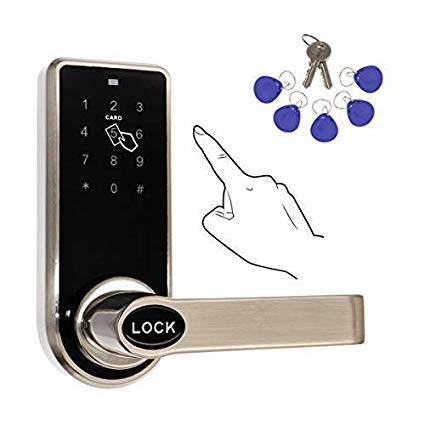
\includegraphics[width=\textwidth]{figures/diagram.jpg}
        \vfill
        \vfill
    \end{titlepage}
\newpage

\section{Objectives}\label{sec:objectives}
At the end of this activity, students will:

\begin{itemize}
\item {Have a basic understanding of how RFID tags work in the context of RFID
    security systems common to many office/apartment buildings. }
\item {Be able to explain why only RFID or only keypad security systems are generally
    not sufficient for reasonable levels of security on their own. }
\end{itemize}

\section{Parts Required}\label{sec:parts}

\begin{itemize}
\begin{minipage}{0.4\linewidth}
    \item Arduino board
    \item Breadboard
    \item Servomotor
    \item LED
    \item MFRC522 RFID reader
\end{minipage}
\begin{minipage}{0.4\linewidth}
    \item I2C LCD
    \item Jumper wires
    \item 220-ohm resistors
    \item Buzzer
    \item 6 to 12V Power source
\end{minipage}
\end{itemize}

\section{Setup}
\begin{enumerate}
\item {Download, unzip, and install the Arduino Integrated Development Environment
    (IDE) from https://www.arduino.cc/en/Main/Donate (does not need admin
    privileges).}
\item {Gather all the necessary parts listed in \ref{sec:parts}}  
\end{enumerate}

\section{How it Works}

\textbf{RFID reader}, a Radio-Frequency IDentification system has three parts:
\begin{itemize}
\item A scanning antenna, which emits tiny amounts of electricity through the air
  that transponders (the RFID tag) can pickup.
\item A transceiver (a circuit that can both send/receive data) with a decoder to
  interpret the data.
\item A transponder (the RFID tag) that has been programmed with a specific numerical
  key unique to it. This key is like a unique sequence of numbers for a combination
  lock, and will only open certain locks that have been programmed to accept its
  unique sequence.
\end{itemize}

RFID tags do not need to contain batteries, and can therefore remain usable for very
long periods of time (years or even decades!). This is one of the reasons why they
are common security features in apartment/office building settings. When an RFID tag
passes through the field of the scanning antenna, the tiny amount of electric current
that is enough ``wake up'' the RFID tag, which will then transmit its ``key'' to the
scanning antenna, which will in turn relay that key to the transceiver on the other
end. If the key in the RFID chip is considered valid by the transceiver, then it will
tell whatever circuit it is attached to that the RFID chip is valid, and the
door/safe/etc. will open.
\\
\\
In our setup, similar to that found at many high security office buildings/banks,
users will have to (1) scan the correct RFID tag, and (2) enter the correct password
on the keypad to be able to unlock the door (a green LED will light up). If you scan
the wrong RFID tag or enter the wrong password, the red LED will light up
instead. You can imagine a buzzer or other security response going off when this
happens!

\newpage
\section{Building the Circuits}
The RFID reader from the parts list above is the transceiver in our setup. It
communicates with the Arduino through the SPI protocol (a special communication
language like German/Mandarin/Hungarian/etc). Follow the steps shown below to
connect the RFID with Arduino.
\\
\\
\begin{enumerate}
\item First plug the board with the RFID transceiver into the breadboard, and connect
  it to the arduino as shown in Fig.~\ref{fig:rfid-lock1}.

  \begin{figure}[H]
  \centering
  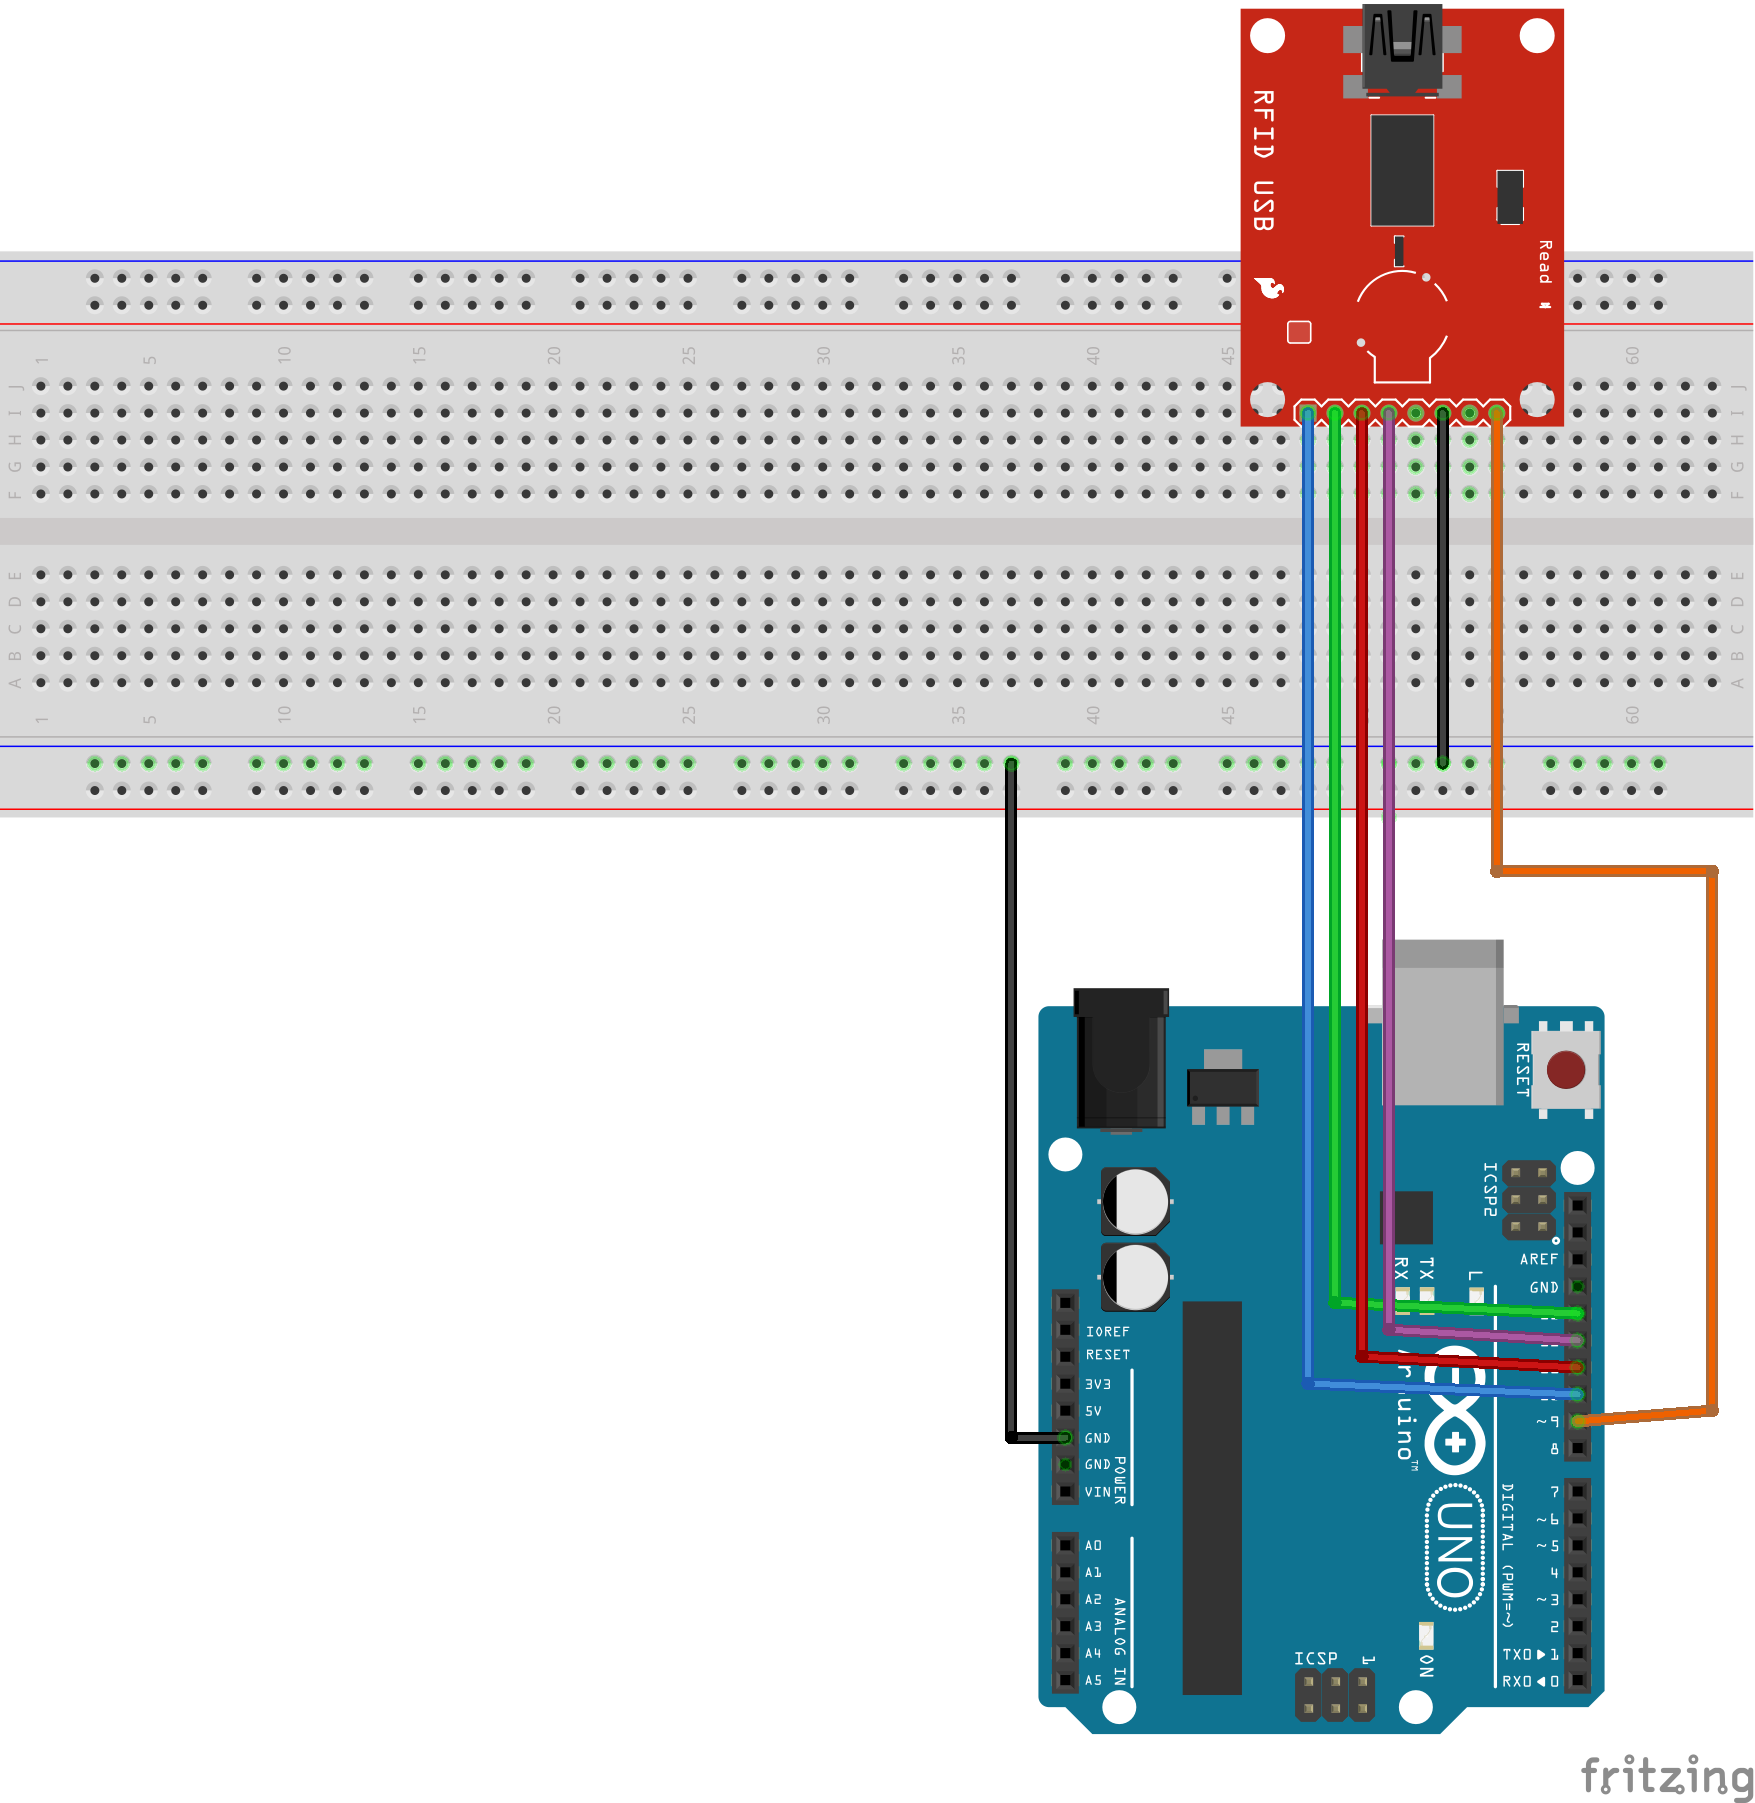
\includegraphics[width=.7\linewidth]{figures/rfid-lock1_bb.png}
  \caption{\label{fig:rfid-lock1}}
\end{figure}

\item Next, connect the RFID transceiver to power on the Arduino as shown in
  Fig.~\ref{fig:rfid-lock2}. Note that it needs to be connected to the 3V output on
  the board, NOT the 5V output we have used for everything else (which is why this is
  its own step).

    \begin{figure}[H]
  \centering
  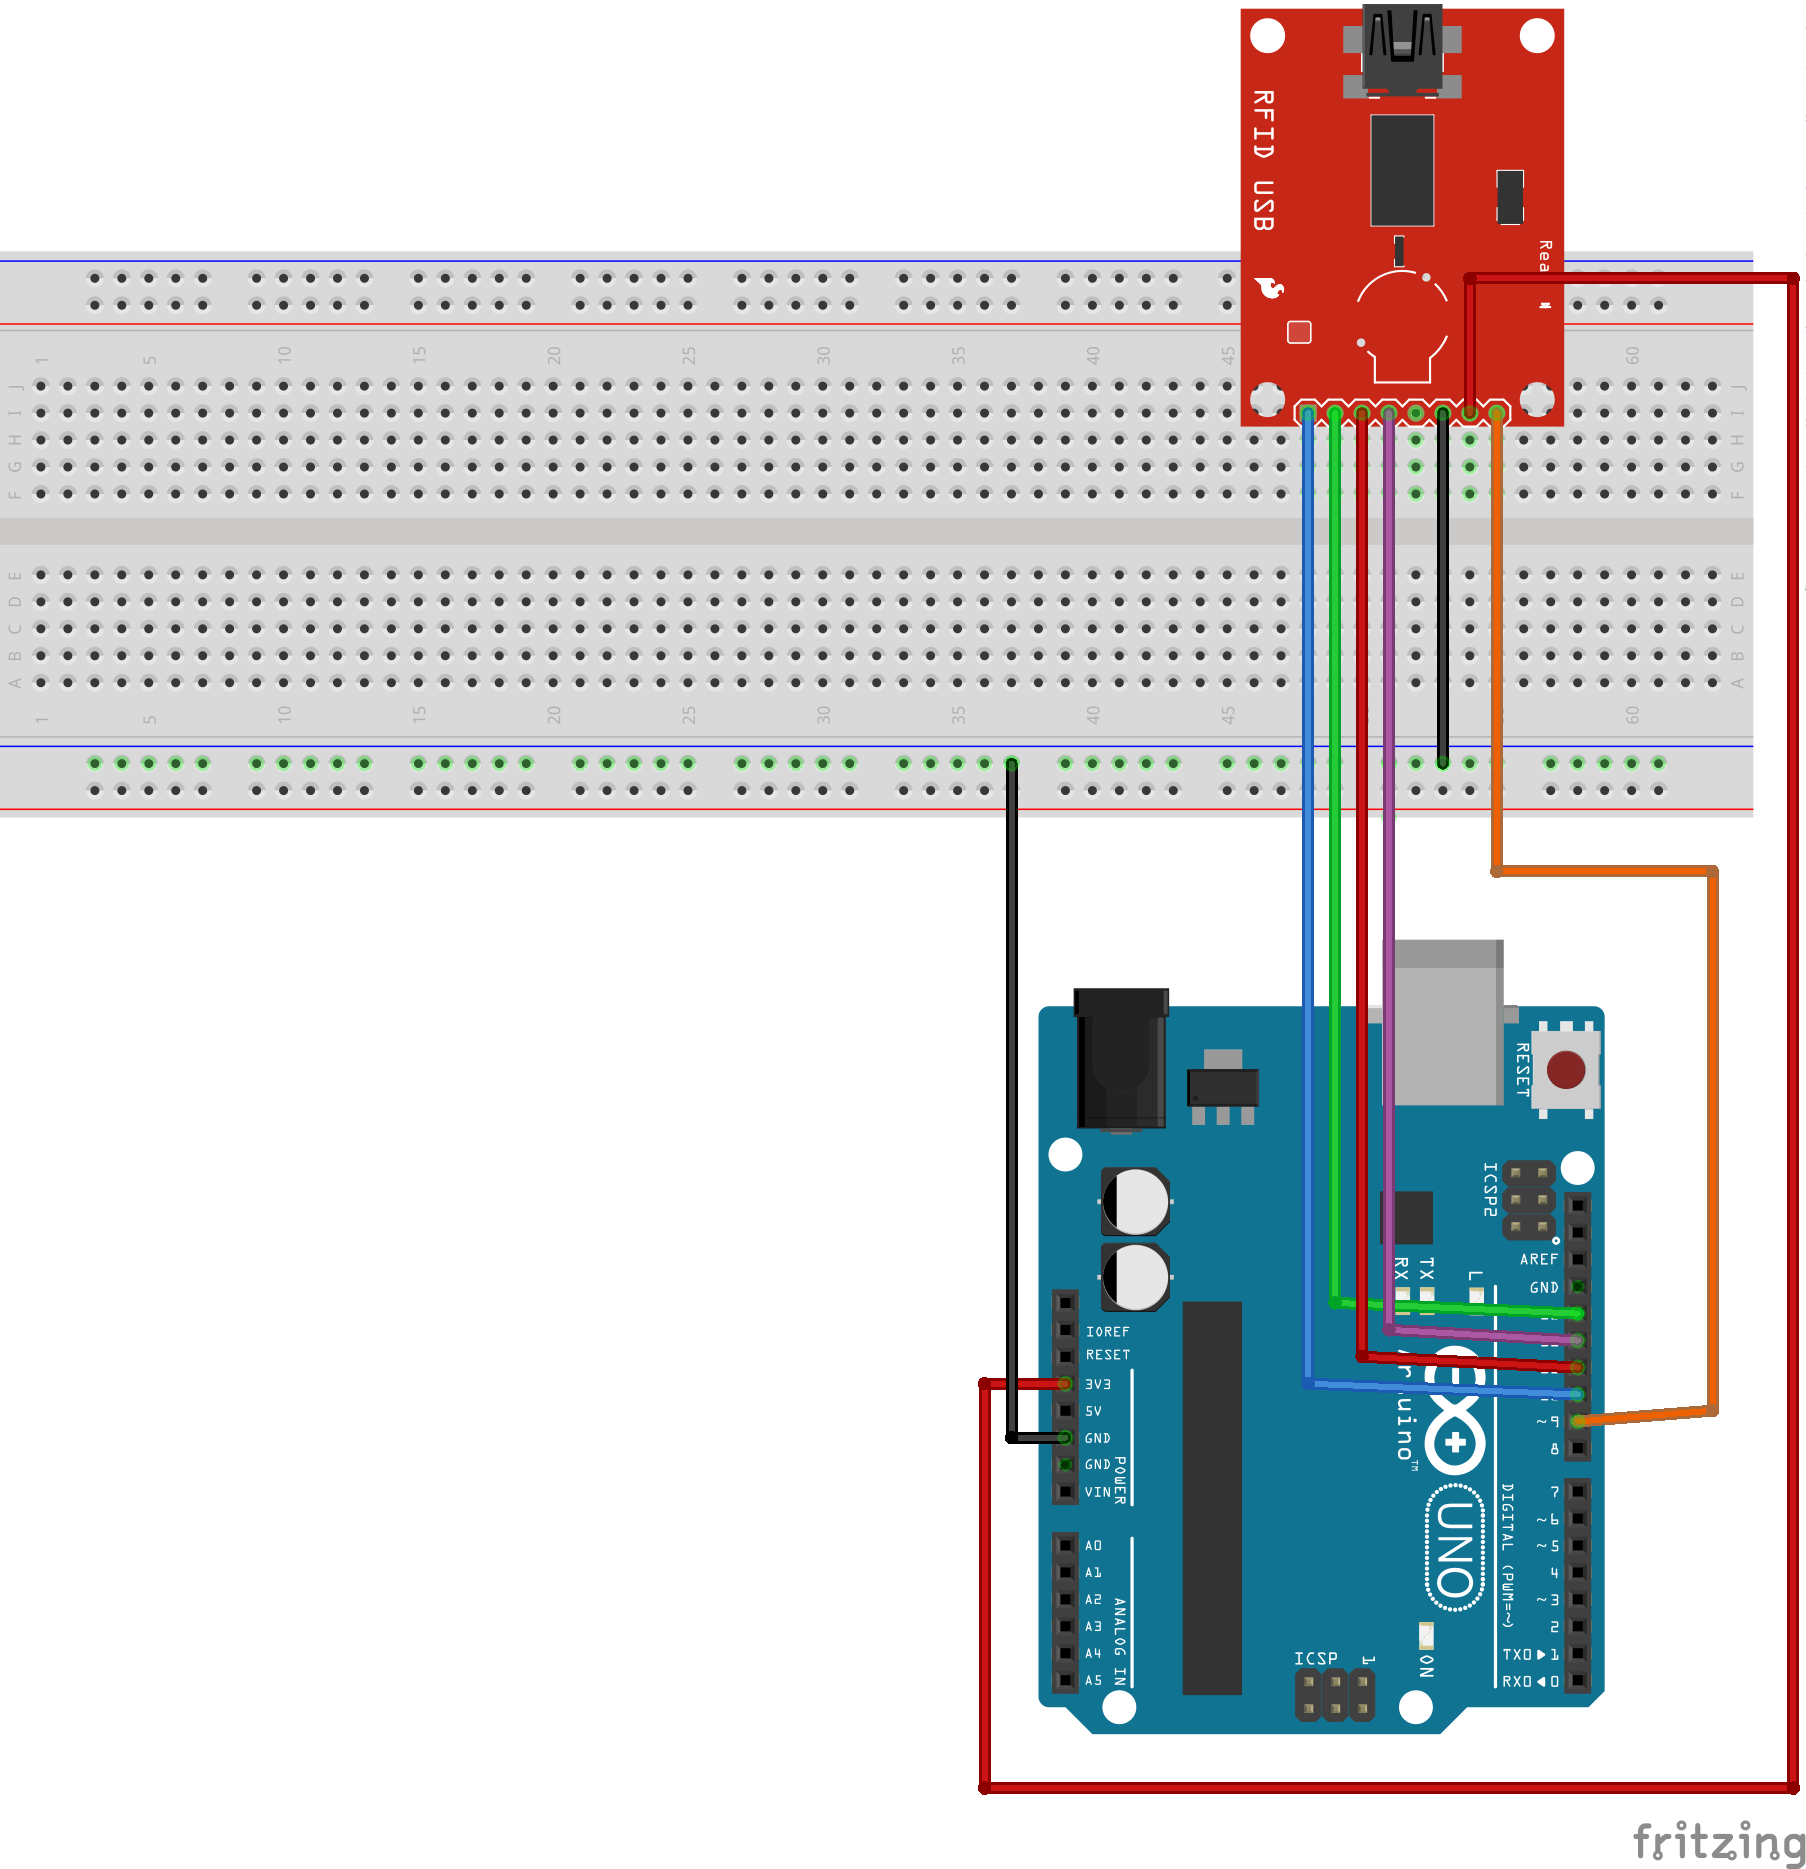
\includegraphics[width=.7\linewidth]{figures/rfid-lock2_bb.png}
  \caption{\label{fig:rfid-lock2}}
\end{figure}

\item Plug the keypad into pins 2-8 on the Arduino as shown in
  Fig.~\ref{fig:rfid-lock3}. The leftmost pin of the keypad should go into pin 8.

  \begin{figure}[H]
  \centering
  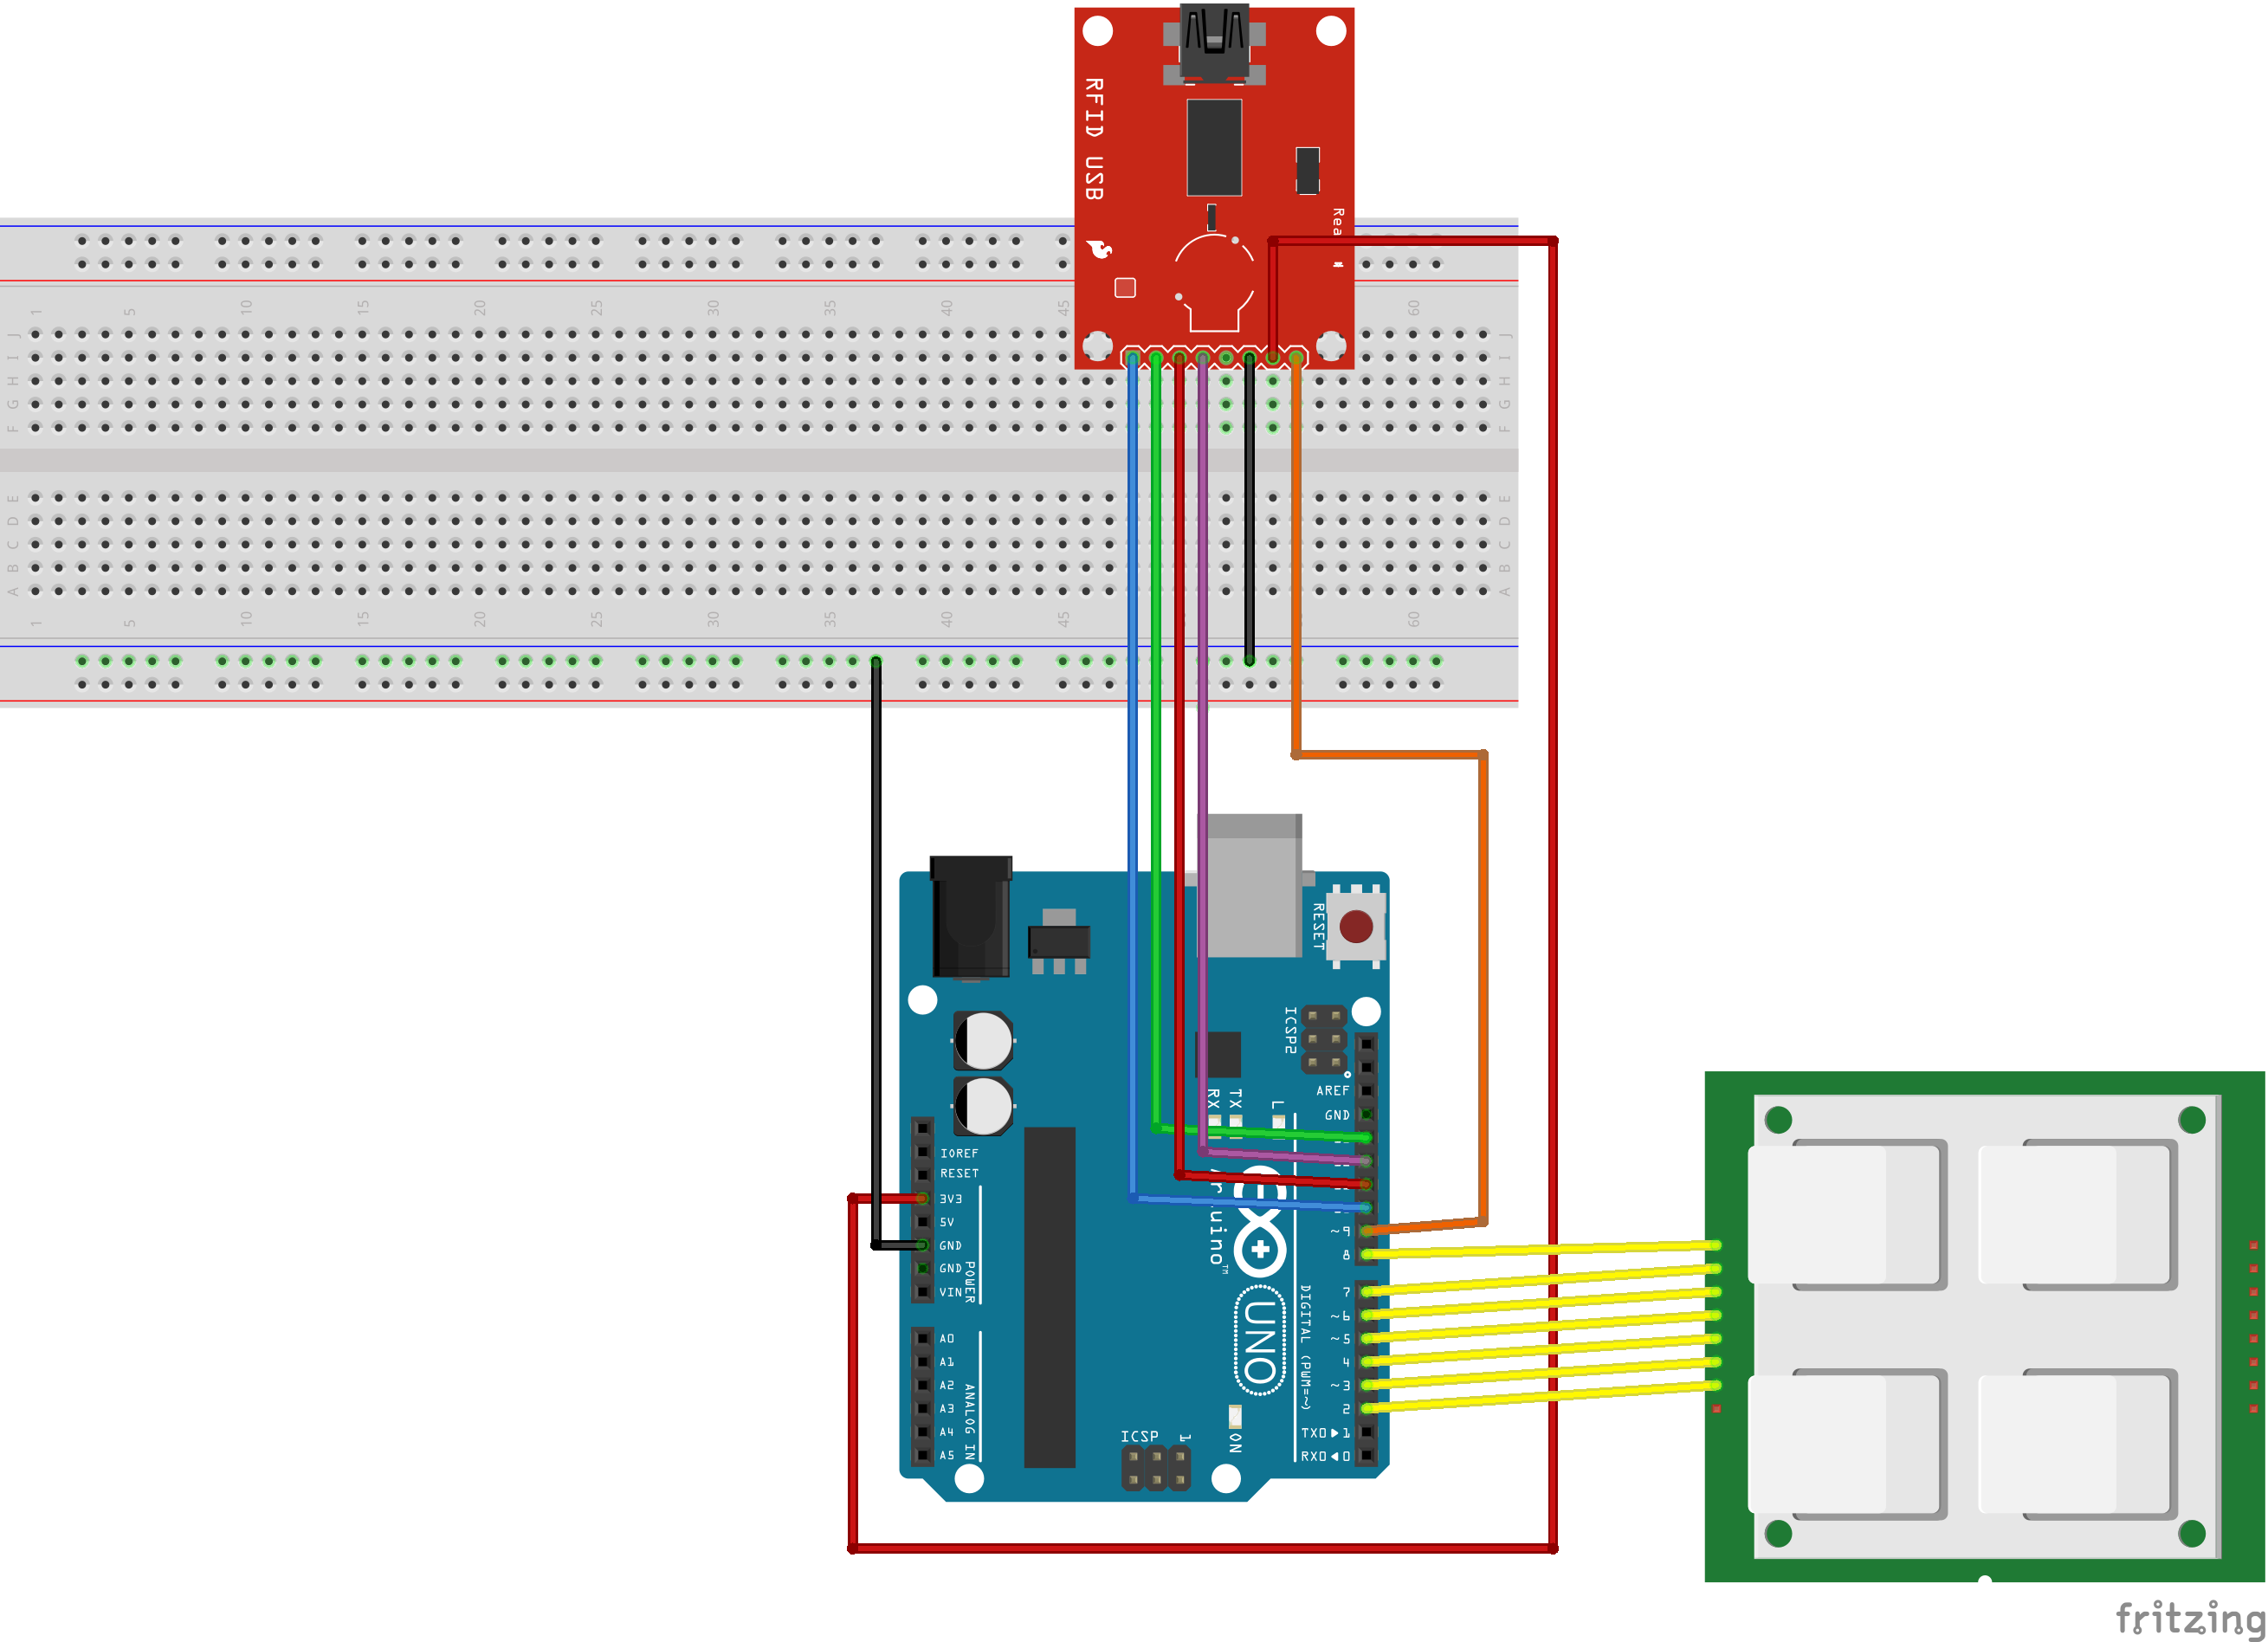
\includegraphics[width=.7\linewidth]{figures/rfid-lock3_bb.png}
  \caption{\label{fig:rfid-lock3}}
\end{figure}

\item Finally, put the green and red LEDs on the board as shown in
  Fig.~\ref{fig:rfid-lock4}.

  \begin{figure}[H]
  \centering
  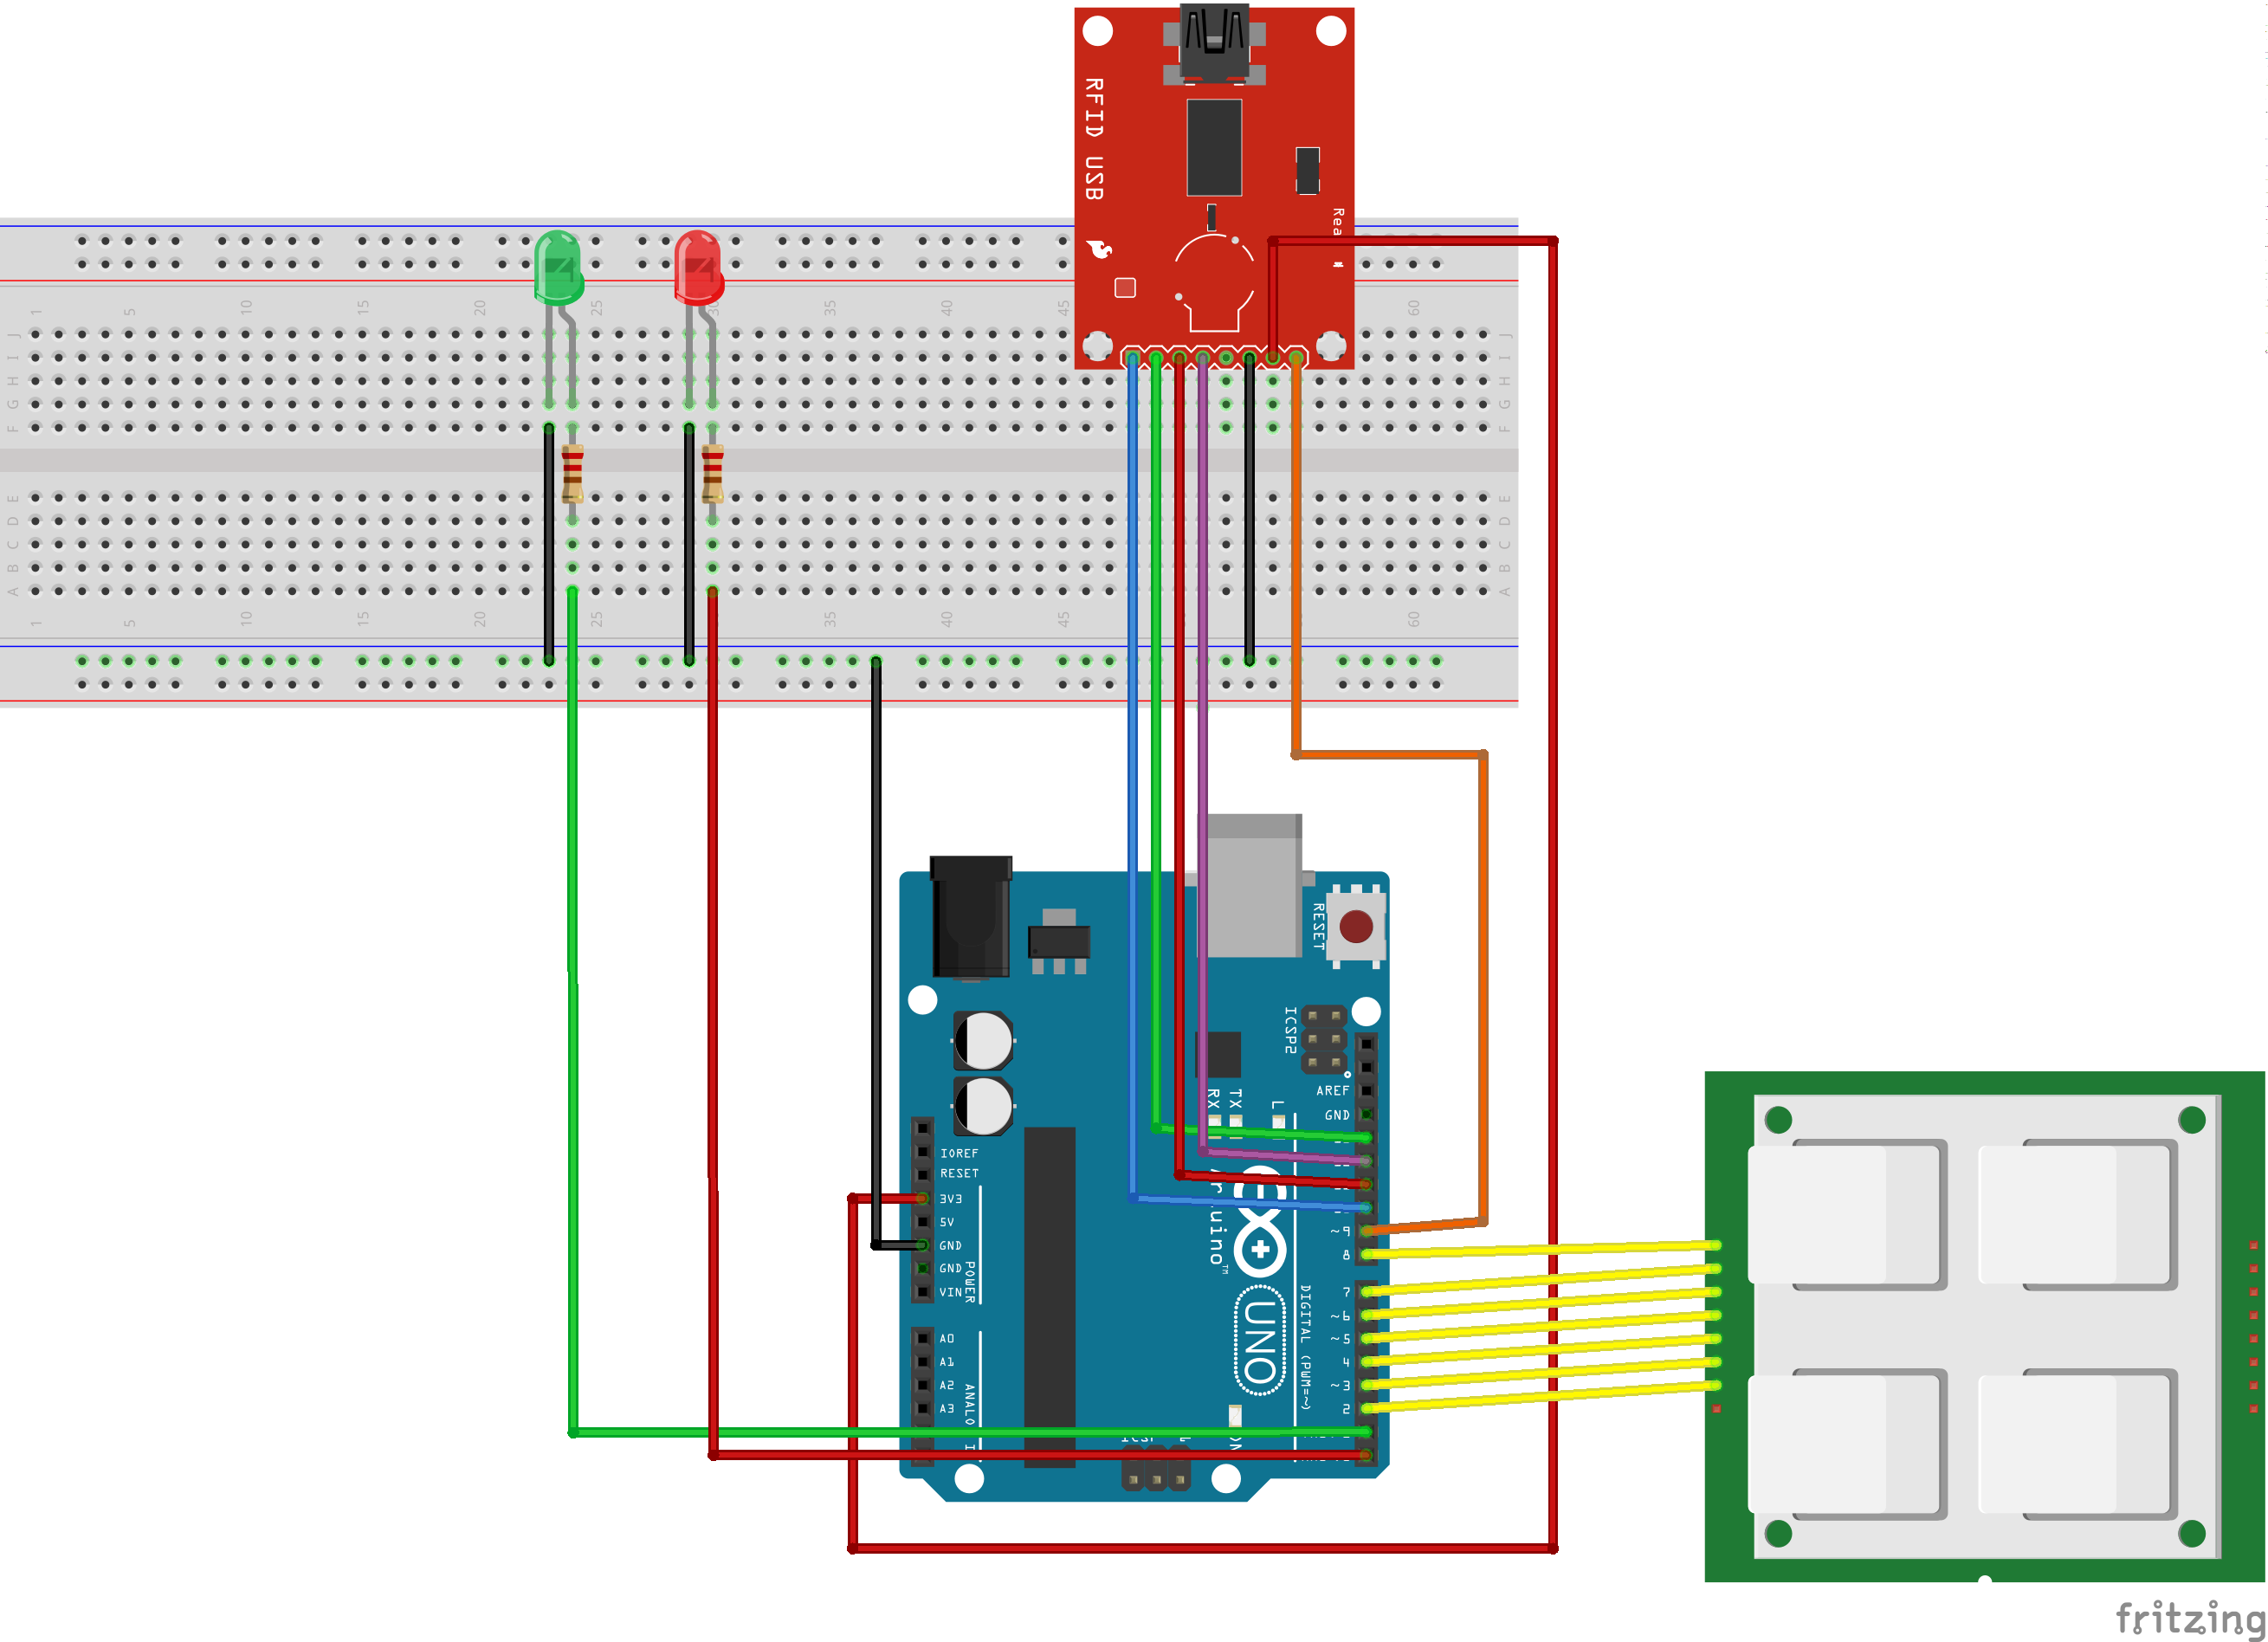
\includegraphics[width=.7\linewidth]{figures/rfid-lock4_bb.png}
  \caption{\label{fig:rfid-lock4}}
\end{figure}

\end{enumerate}

\section{Programming the Arduino}
The base code for programming the Arduino is provided. Using the Arduino IDE, open
the .ino file.  The IDE allows you to do 4 things: edit the code, verify the code
(i.e. does not contain syntax errors), upload the code to the Arduino, and view the
diagnostic output of things as they run on the Arduino.  Uploading to the Arduino is
easy! Just click the Upload arrow in the IDE.

As you have learned, each RFID chip has its own universal unique ID (UUID), so we
need to tell the transceiver attached the Arduino about the unique key before the
fob/card will be accepted. <TODO: finish this...>

\section{Extending the Code}
The initial password is ‘1234’.
\\
Change the tag’s UID in the below line of code with your tag’s UID.
\\
\textbf{String tagUID = “29 B9 ED 23”;}

\end{document}
